\documentclass{article}
\usepackage[margin=1in]{geometry}
\usepackage{amsmath, amssymb, amsfonts}
% change equation numbering to section.eq_num
\numberwithin{equation}{section}
% set paragraph indent
\setlength\parindent{0pt}
% makes clickable links to sections
\usepackage{hyperref}
% make the link colors blue, as well as cite colors
\hypersetup{colorlinks, linkcolor=blue, citecolor=blue, urlcolor=magenta}
\usepackage{pgfplots}
% text tilde. see https://tex.stackexchange.com/a/9372/234752
% note: pdflatex complains that \texttilde already defined
% note: unused because this is just too much work
\usepackage{textcomp}
\newcommand{\mytexttilde}{\raisebox{0.5ex}{\texttildelow}}

% C++ command. use typewriter text to make the + not so big
\newcommand{\CXX}{C\texttt{++}}

\title{Estimating $ \pi $ with quasi-Monte Carlo}
\author{Derek Huang}
\date{November 3, 2025}

\begin{document}

\maketitle

\section{Introduction}

A well-known introduction to Monte Carlo methods is the estimation of $ \pi $
using Monte Carlo. Essentially, the Monte Carlo method is used to approximate
the following integral over $ [0, 1] $:

\begin{equation} \label{pi_integral}
    \int_0^1\sqrt{1 - x^2}dx
\end{equation}

This integral is exactly $ \frac{1}{4} $ the area of the unit-radius circle and
so $ \pi $ can be estimated as follows:

\begin{enumerate}
    \item
    Construct $ S_n \triangleq \{(x_1, y_1), \ldots (x_n, y_n)\} \in [0, 1]^2 $

    \item
    Determine $ I_n \triangleq \{(x, y) \in S_n : x^2 + y^2 \le 1 \} $

    \item
    Obtain the $ \pi $ estimator $ \hat{\pi}_n \triangleq \frac{4|I_n|}{n} $
\end{enumerate}

From an algorithmic standpoint steps 2 and 3 are quite simple and have little
room for interpretation. The main difficulty is step 1, as ``construct'' in
this context means to sample points in $ [0, 1]^2 $ using Monte Carlo. Usually
this entails using a pseudo-random number generator (PRNG) algorithm like the
32- or 64-bit Mersenne Twister, Philox, etc. to construct $ S_n $, but
low-discrepancy sequences, e.g. Halton, or more commonly, Sobol, may be used.
The latter would be referred to as quasi-Monte Carlo.

\medskip

However, estimating (\ref{pi_integral}) with Monte Carlo requires an inordinate
amount of samples for even a poor estimate. Although in general quasi-Monte
Carlo promises better accuracy, it still suffers when the integrand dimension
is high. In the case of Sobol sequences, selection of the direction numbers is
crucial for constructing a good low-discrepancy sequence, and requires a large
amount of state.

\section{Stratification}

Let's take a step back and consider the goal of using low-discrepancy sequences
in quasi-Monte Carlo. Compared to using a PRNG in Monte Carlo, the
low-discrepancy sequence promises a deterministic way to ``evenly'' cover the
area of integration, e.g. $ [0, 1]^n $ in the classical construction. For our
estimation of $ \pi $, we only care about $ [0, 1]^2 $, which is of course easy
for us to visualize. In this case, one might consider the most na\"ive method
of constructing a $ S_n $ that ``evenly'' covers $ [0, 1]^2 $, namely

\begin{equation} \label{sn_stratified}
    \tilde{S}_{\nu^2} \triangleq
    \left\{
        \left(\frac{i + \frac{1}{2}}{\nu}, \frac{j + \frac{1}{2}}{\nu}\right)
        \in [0, 1]^2 : i, j \in \{0, \ldots \nu - 1\}
    \right\}
\end{equation}

The set $ \tilde{S}_{\nu^2} $ defines an evenly-spaced grid of
$ n \triangleq \nu^2 $ points such that
$ \forall \mathbf{x} \in \tilde{S}_{\nu^2} $,
$ \exists i, j \in \{0, \ldots \nu - 1\} $ such that $ \mathbf{x} $ is the
centroid of the points $ \left(\frac{i}{\nu}, \frac{j}{\nu}\right) $,
$ \left(\frac{i}{\nu}, \frac{j + 1}{\nu}\right) $,
$ \left(\frac{i + 1}{\nu}, \frac{j}{\nu}\right) $,
$ \left(\frac{i + 1}{\nu}, \frac{j + 1}{\nu}\right) $.
As shown in Figure \ref{stratified_qmc_pi}, this scheme is essentially the
rectangle rule in two dimensions, constructed such that all points in
$ \tilde{S}_{\nu^2} $ are strictly within $ (0, 1)^2 $ and are centroids of the
``natural'' rectangle rule points whose coordinate values are multiples of
$ \frac{1}{\nu} $.

\begin{figure}
    \centering
    % nu = 10
    % TODO: could be a macro but i don't know how to do that
    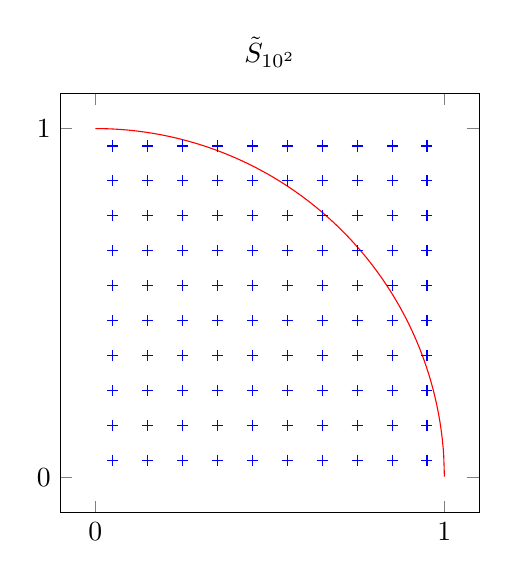
\begin{tikzpicture}
        \begin{axis}[
            title=$ \tilde{S}_{10^2} $,
            width=8cm,
            % fix axis ranges
            xmin=-0.1,
            xmax=1.1,
            ymin=-0.1,
            ymax=1.1,
            % only want endpoints
            xtick={0, 1},
            ytick={0, 1},
            % by default you'd need to tilt your head to read the y label
            y label style={rotate=-90},
            % ensure axis aspect ratio is 1:1
            axis equal image,
            clip=false
        ]
        % plot of upper right quadrant of unit circle on [0, 1]
        % note: need more samples otherwise graph doesn't touch x=1 enough
        \addplot[domain=0:1, samples=500, color=red, smooth]{sqrt(1 - x^2)};
        % plot the rectangle rule grid points
        \foreach \xvalue in {0.0, 0.1, ..., 1.0} {
            \foreach \yvalue in {0.0, 0.1, ..., 1.0} {
                % use \edef trick to expand loop variables but not \addplot
                % see https://tex.stackexchange.com/a/71199/234752
                \edef\gridpoint{
                    \noexpand\addplot[color=blue, mark=+] coordinates {
                        (\xvalue + 0.05, \yvalue + 0.05)
                    };
                }
                % invoke macro
                \gridpoint;
            }
        }
        \end{axis}
    \end{tikzpicture}
    % nu = 20
    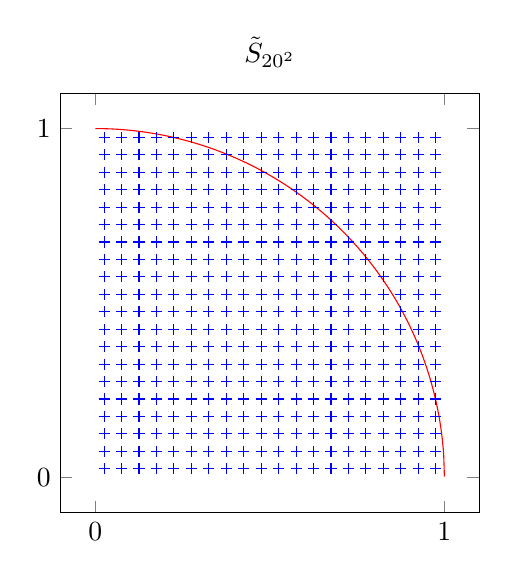
\begin{tikzpicture}
        \begin{axis}[
            title=$ \tilde{S}_{20^2} $,
            width=8cm,
            % fix axis ranges
            xmin=-0.1,
            xmax=1.1,
            ymin=-0.1,
            ymax=1.1,
            % only want endpoints
            xtick={0, 1},
            ytick={0, 1},
            % by default you'd need to tilt your head to read the y label
            y label style={rotate=-90},
            % ensure axis aspect ratio is 1:1
            axis equal image,
            clip=false
        ]
        % plot of upper right quadrant of unit circle on [0, 1]
        % note: need more samples otherwise graph doesn't touch x=1 enough
        \addplot[domain=0:1, samples=500, color=red, smooth]{sqrt(1 - x^2)};
        % plot the rectangle rule grid points
        % note: tried 50 x 50 points and that resulted in very slow compile.
        % the 20 x 20 points already slows down compile a lot
        \foreach \xvalue in {0.0, 0.05, ..., 1.0} {
            \foreach \yvalue in {0.0, 0.05, ..., 1.0} {
                % use \edef trick to expand loop variables but not \addplot
                \edef\gridpoint{
                    \noexpand\addplot[color=blue, mark=+] coordinates {
                        (\xvalue + 0.025, \yvalue + 0.025)
                    };
                }
                % invoke macro
                \gridpoint;
            }
        }
        \end{axis}
    \end{tikzpicture}
    \caption{
        Points of $ \tilde{S}_{\nu^2} $ and plotted over $ \sqrt{1 - x^2} $ for
        $ \nu = 10 $ and $ \nu = 20 $.
    }
    \label{stratified_qmc_pi}
\end{figure}

\medskip

Of practical importance is the fact that constructing $ \tilde{S}_{\nu^2} $ is
incredibly cheap compared to other methods of constructing $ S_n $, whether it
be via pseudorandom or quasirandom sequences of points sampled from
$ [0, 1]^2 $. For example, a straightforward \CXX{} implementation that uses
the points of  $ \tilde{S}_{\nu^2} $, where $ \nu \triangleq 10^3 $, i.e.
$ n \triangleq 10^6 $, ran in only 2 ms. In comparison, a cuRAND implementation
using the provided 32-bit Mersenne Twister implementation took around 141 ms.
Of course, the estimator accuracy left much to be desired, but since the
rectangle rule sampling approach is very cheap, even sampling 25 million
points, i.e. with $ \nu \triangleq 5 \times 10^3 $, took only around 66 ms, and
with compiler%
\footnote{Compiler used is GCC 11.3.0 on WSL1 Ubuntu 22.04.2 LTS.}
optimization, took only 22 ms or so to complete.

\medskip

TODO: Work in progress. Will discuss SIMD later (3 ms runtime) and need pictures.

\end{document}
